\chapter{物理のための微分・積分}
\label{differentialequation}
力学に限らず物理では頻繁に微分方程式というものを解きます。ここではその中でも力学によく出てくるものの紹介と基本的な解き方を解説します。簡単に言ってしまえば、力学で解く微分方程式は(多分)運動方程式だけです。運動方程式といえば、

\begin{equation}
    ma = F \notag
\end{equation}

を思い浮かべるかもしれませんが、これからはこう書くことにしましょう。

\begin{equation}
    m\frac{\mathrm{d^2}\bm{r}}{\mathrm{d}t^2} = \bm{F} \notag
\end{equation}

または、

\begin{equation}
    m\ddot{\bm{r}} = \bm{F} \notag
\end{equation}



ここで、演算子$\mathrm{d^2}\bm{r}/\mathrm{d}t^2$と$\ddot{\bm{r}}$は両者とも同じ意味で、位置$\bm{r}$を時間$t$で2回微分した形です。物理では、何かの関数を時間$t$で微分した際、その階数だけ関数の上にドットをつける習慣があります\footnote{微分を$n$回行うことを$n階$と言います。しかし、決して$n$回微分と言うことはありません。読みが同じで紛らわしいです。}。

力学的な現象は基本的にこのように、微分された関数が含まれた形で記述されます。私たちはこの方程式を「解く」ことで、自然現象を理解していきます。実際にこれを解くのは\ref{differentialequation-figureseries}節まで待って、ここでは微分、積分が一体何者なのかをお話しましょう。




\section{微分}
\label{differential}
実は歴史的には積分の方が微分よりも圧倒的に早く発明されたのですが、通例では微分を先に学びます。本書でもその流れで説明していきます。

「AをBで微分する」は、簡単に言うとAを縦軸、Bを横軸にとったグラフの傾きとBを対応させた関数を求めることに当たります。微分の視覚的なイメージを図\ref{fig:differential}に示します。

\begin{figure}[htbp]
\begin{center}
\begin{minipage}{0.4\hsize}
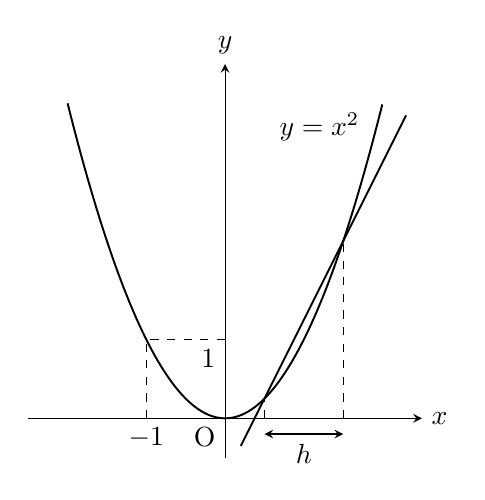
\begin{tikzpicture}[domain=-2:2,samples=300,>=stealth]
   % 座標軸
   \draw[->] (-2.5,0) -- (2.5,0) node[right] {$x$};
   \draw[->] (0,-0.5) -- (0,4.5) node[above] {$y$};
   \node [anchor=north east] at (0,0) {O};
 
   \draw[line width=0.7pt] plot (\x,{\x*\x});
   \node [anchor=north] at (1.2,4){$y=x^2$};
   
   % 補助線
   \draw [dashed](0,1) node [anchor=north east]{$1$}--(-1,1);
   %\draw [dashed](0,1)--(-1,1);
   %\draw [dashed](1,0) node [anchor=north]{$1$}--(1,1);
   \draw [dashed](-1,0) node [anchor=north]{$-1$}--(-1,1);
   \draw [dashed](0.5,0)--(0.5,{0.5^2});
   \draw [dashed](1.5,0)--(1.5,{1.5^2});
   \draw [<->](0.5,-0.2)--(1.5,-0.2);
   \node [anchor=north] at (1,-0.2){$h$};
   
   \draw[line width=0.7pt, domain = 0.2:2.3] plot (\x,{(2.25-0.25)/(1.5-0.5)*(\x-1.5)+2.25});
 
\end{tikzpicture}
\end{minipage}
\begin{minipage}{0.4\hsize}
\begin{tikzpicture}[domain=-1.5:1.5,samples=300,>=stealth]
   % 座標軸
   \draw[->] (-2.5,0) -- (2.5,0) node[right] {$x$};
   \draw[->] (0,-3.5) -- (0,3.5) node[above] {$y$};
   \node [anchor=north west] at (0,0) {O};
 
   \draw[line width=0.7pt] plot (\x,{2*\x});
   \node [anchor=north] at (1,4){$y=2x$};
   
   % 補助線
   \draw [dashed](0,2) node [anchor=east]{$2$}--(1,2);
   \draw [dashed](0,-2) node [anchor=west]{$-2$}--(-1,-2);
   \draw [dashed](1,0) node [anchor=north]{$1$}--(1,2);
   \draw [dashed](-1,0) node [anchor=south]{$-1$}--(-1,-2);
 
\end{tikzpicture}
\end{minipage}
\caption{左: 微分のイメージ、右: 導関数}
\label{fig:differential}
\end{center}
\end{figure}

なお、ある関数Aを微分をした関数Bを「関数Aの導関数」と言います。

ここで微分の定義を確認しましょう。

微分はグラフの傾きを表す関数だと先程書きました。$f(x)-x$グラフの、ある区間$[x,x+h]$での(平均の)傾き$s(x)$は以下のように表せます。ここで、$h>0$です。

\begin{eqnarray}
    s(x) &=& \frac{f(x+h)-f(x)}{(x+h)-x} \notag \\
    &=&\frac{f(x+h)-f(x)}{h} \notag
\end{eqnarray}

これはあくまでも「平均の」傾きで、グラフの傾きを正確に表しているとは言えません。これを正確にしていくためには$h$を$0$に近づけていけば良さそうです。

\begin{eqnarray}
    \frac{\mathrm{d}}{\mathrm{d}x}f(x) = \lim_{h\to 0}\frac{f(x+h)-f(x)}{h}
    \label{eq:differential-def}
\end{eqnarray}

ここで記号$\lim_{h\to 0}$は、$h$を限りなく$0$に近づける\footnote{本来の定義では$h$は正の方向から$0$に近づけるべきですが、よく考えると負の方向から近づけた場合も同じ式の形で正確に定義できることがわかります。}ことを示しています\footnote{$\lim$の記号には、変数をある数値、または$+\infty$、$-\infty$に極限まで近づけるという意味があります。何を何に近づけるかは記号の下に表記します。なお、近づける数値に正の方向から近づけるのか、負の方向から近づけるのかを指定する際にはそれぞれ$+0$、$-0$をつけて表現します。}。これが正確な微分の定義です。

表\ref{tab:differential}に一般的な関数の微分に関する公式を示します。なお、導関数は微分したあとの関数です。なぜこうなるか気になった方は各自調べるなり微分の定義式を使って計算してみるなりしてみてください。

\begin{table}[htb]
 \begin{center}
  \caption{微分に関する公式(それぞれ$x$で微分)}
  \label{tab:differential}
  \begin{tabular}{l|l}
    \hline
    関数 & 導関数 \\
    \hline \hline
    $x^n$ & $nx^{n-1}$ \\
    $\sin x$ & $\cos x$ \\
    $\cos x$ & $-\sin x$ \\
    $\tan x$ & $1/\cos^2x$ \\
    $a^x$ & $a^x\log a$ \\
    $\log_ax$ & $1/(x\log a)$ \\
    
  \end{tabular}
 \end{center}
\end{table}


微分した関数の表記について、一般的に以下のような記号が使われます。左は位置$x$を時間$t$で微分した関数で、右は左の関数を更に時間$t$で微分した関数($t$での2階微分)を表します。

\begin{eqnarray}
    \frac{\mathrm{d}x}{\mathrm{d}t} \notag ,\ 
    \frac{\mathrm{d^2}x}{\mathrm{d}t^2} \notag
\end{eqnarray}

また、くどいようですが、いちいちこのような形で書くのは面倒なので、物理では特に何かの関数(ここでは位置$x$)の時間微分について、

\begin{eqnarray}
    \frac{\mathrm{d}x}{\mathrm{d}t} &=& \dot{x} \notag \\
    \frac{\mathrm{d^2}x}{\mathrm{d}t^2} &=& \ddot{x} \notag
\end{eqnarray}

というように、ドットを上につけて表すことが多々あります\footnote{本書では、$\mathrm{d}x/\mathrm{d}t$等と書いたほうがわかりやすい場合はそう書くことにします。}。


\subsection{合成関数の微分}
\label{differential-composite}
\ref{function}節でも少しお話ししましたが、「合成関数」とは、関数の入力に関数が使われている状態(全体の関数)のことです。仮に関数$f(x)$の入力に関数$g(x)$を使ったとしてみましょう。これを$x$で微分するとき、微分の記号$\mathrm{d}/\mathrm{d}x$を分数のように考えて、以下のように考えられます。

\begin{eqnarray}
    \frac{\mathrm{d}}{\mathrm{d}x}f(g(x)) &=& \frac{\mathrm{d}}{\mathrm{d}g(x)}\frac{\mathrm{d}g(x)}{\mathrm{d}x}f(g(x)) \notag \\
    &=& \frac{\mathrm{d}}{\mathrm{d}g(x)}f(g(x))\times \frac{\mathrm{d}g(x)}{\mathrm{d}x}
\end{eqnarray}

この式は、$f(g(x)$を$x$で微分したものは、$f(g(x))$を$g(x)$で微分したものに$g(x)$を$x$で微分したものをかけ合わせることで計算できるということを表します。これは「合成関数の微分」と呼ばれます\footnote{この証明は現段階ではかなり直感的なもので、まず微分の記号が分数のように扱えることを本来は証明すべきです。ですがこれに関しては$\epsilon-\delta$論法を学ばないとよく理解できないため、(この本は数学書ではないこともあり、)ここでは割愛します。}。

\subsection{積の微分}
\label{differential-product}
ここでは関数の積$f(x)g(x)$を$x$で微分してみましょう。今回は微分の定義式である式(\ref{eq:differential-def})を用いて考えます。二行目で少しトリッキーな変形をしますが、こうすると扱いにくかった$f(x+h)g(x+h)$が扱いやすくなります。

\begin{eqnarray}
    \frac{\mathrm{d}}{\mathrm{d}x}(f(x)g(x)) &=& \lim_{h\to 0}\frac{f(x+h)g(x+h)-f(x)g(x)}{h} \notag \\
    &=& \lim_{h\to 0}\frac{f(x+h)g(x+h)-f(x+h)g(x)+f(x+h)g(x)-f(x)g(x)}{h} \notag \\
    &=& \lim_{h\to 0}\left(\frac{g(x+h)-g(x)}{h}f(x+h)\right)+\lim_{h\to 0}\left(\frac{f(x+h)-f(x)}{h}g(x+h)\right) \notag \\
    &=& \frac{\mathrm{d}}{\mathrm{d}x}g(x)\times f(x)+\frac{\mathrm{d}}{\mathrm{d}x}f(x)\times g(x)
\end{eqnarray}

これは積の微分と呼ばれます。



\subsection{逆関数の微分}
\label{differential-inverse}
逆関数は例えば$y=f(x)$という関数に対し、同値な関数を$x=g(y)$と表記したもので、$g(x)=f^{-1}(y)$と書きます。また、逆関数は$x-y$平面にグラフを描くと互いに$y=x$に対称になっています。

逆関数は元の関数と$y=x$に対称です。よって、ある点での逆関数の傾きは元の関数のその点に対応する傾きの逆数です。例として図\ref{fig:inverse}を参照してください。

\begin{figure}[htbp]
\begin{center}
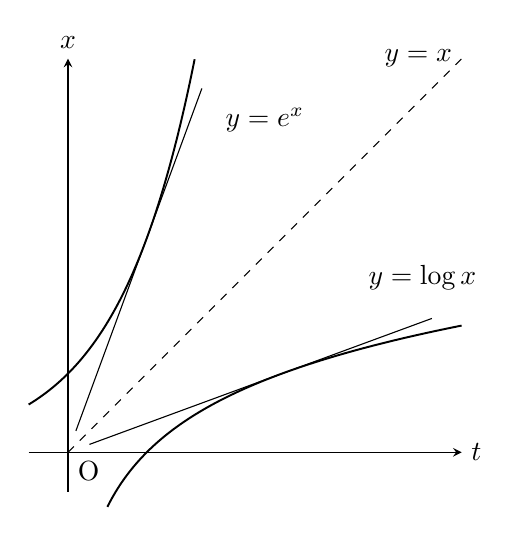
\begin{tikzpicture}[domain=-0.5:5,samples=300,>=stealth]
   % 座標軸
   \draw[->] (-0.5,0) -- (5,0) node[right] {$t$};
   \draw[->] (0,-0.5) -- (0,5) node[above] {$x$};
   \node [anchor=north west] at (0,0) {O};
 
   \draw[line width=0.7pt,domain=-0.5:1.61] plot (\x,{e^\x});
   \node [anchor=north] at (2.5,4.5){$y=e^x$};
   \draw[line width=0.7pt,domain=0.5:5] plot (\x,{ln(\x)});
   \node [anchor=north] at (4.5,2.5){$y=\log x$};
   
   \draw [solid](0.1,0.1*e)--(1.7,e*1.7);
   \draw [solid](0.1*e,0.1)--(e*1.7,1.7);
   
   % 補助線
   \draw [dashed](0,0)--(5,5) node [anchor=east]{$y=x$};
 
\end{tikzpicture}
\caption{逆関数とその接線の例}
\label{fig:inverse}
\end{center}
\end{figure}

よって、直感的ではありますが、逆関数の微分公式として以下が言えます。

\begin{eqnarray}
    \frac{\mathrm{d}}{\mathrm{d}x}f^{-1}(x)=\frac{1}{\frac{\mathrm{d}}{\mathrm{d}x}f(x)}
\end{eqnarray}





\section{積分}
\label{integral}
結論から言うと積分の演算は微分の逆操作です。歴史的には微分よりずっと前に積分が考案され、その後微分の考案、そのタイミングでこれらの演算の相互関係が発見されました。

積分はグラフの囲む面積を求めること、と定義することができます。その演算は図\ref{fig:integral}のように、グラフを細かく短冊状に区切っていき、1つずつ足し合わせていくことで行います。

図\ref{fig:integral}を見ると、短冊と関数の間に隙間(誤差)があることがわかると思います。この誤差を減らすために、昔の人は隙間を三角形で近似して、その三角形の面積を算出したりしました。現在では、図の$1/N$を極限まで$0$に近づけることで誤差を$0$に極限まで近づけます。

\clearpage

\begin{figure}[htbp]
\begin{center}
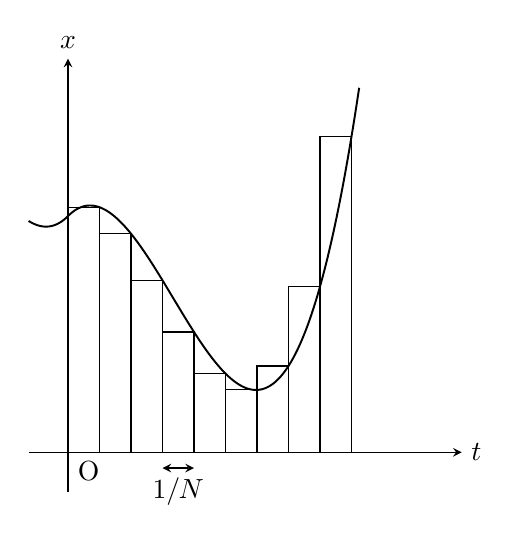
\begin{tikzpicture}[domain=-0.5:5,samples=300,>=stealth]
   % 座標軸
   \draw[->] (-0.5,0) -- (5,0) node[right] {$t$};
   \draw[->] (0,-0.5) -- (0,5) node[above] {$x$};
   \node [anchor=north west] at (0,0) {O};
 
   \draw[line width=0.7pt,domain=-0.5:3.7] plot (\x,0.5*\x^3-2*\x^2+\x+3);
   %\node [anchor=north] at (2.5,4.5){$y=x^3-2x^2+x+2$};
   
   \draw [solid](0,0)--(0,0.5*0.4^3-2*0.4^2+0.4+3)--(0.4,0.5*0.4^3-2*0.4^2+0.4+3)--(0.4,0);
   \draw [solid](0.4,0)--(0.4,0.5*0.8^3-2*0.8^2+0.8+3)--(0.8,0.5*0.8^3-2*0.8^2+0.8+3)--(0.8,0);
   \draw [solid](0.8,0)--(0.8,0.5*1.2^3-2*1.2^2+1.2+3)--(1.2,0.5*1.2^3-2*1.2^2+1.2+3)--(1.2,0);
   \draw [solid](1.2,0)--(1.2,0.5*1.6^3-2*1.6^2+1.6+3)--(1.6,0.5*1.6^3-2*1.6^2+1.6+3)--(1.6,0);
   \draw [solid](1.6,0)--(1.6,0.5*2^3-2*2^2+2+3)--(2,0.5*2^3-2*2^2+2+3)--(2,0);
   \draw [solid](2,0)--(2,0.5*2.4^3-2*2.4^2+2.4+3)--(2.4,0.5*2.4^3-2*2.4^2+2.4+3)--(2.4,0);
   \draw [solid](2.4,0)--(2.4,0.5*2.8^3-2*2.8^2+2.8+3)--(2.8,0.5*2.8^3-2*2.8^2+2.8+3)--(2.8,0);
   \draw [solid](2.8,0)--(2.8,0.5*3.2^3-2*3.2^2+3.2+3)--(3.2,0.5*3.2^3-2*3.2^2+3.2+3)--(3.2,0);
   \draw [solid](3.2,0)--(3.2,0.5*3.6^3-2*3.6^2+3.6+3)--(3.6,0.5*3.6^3-2*3.6^2+3.6+3)--(3.6,0);
   
   \draw [<->](1.2,-0.2)--(1.6,-0.2);
   \node [anchor=north] at (1.4,-0.2){$1/N$};
\end{tikzpicture}
\caption{積分(定積分)のイメージ}
\label{fig:integral}
\end{center}
\end{figure}

積分の定義式(厳密には区分求積法と呼びます)を書いておきます。なお、これは定積分(ある区間の、グラフで囲まれた部分の面積を求めること)の公式です。$\sum$内が一つの短冊の面積で、$f(i/N)$が高さ、$1/N$が横幅です。


\begin{eqnarray}
    F(x) = \lim_{N\to\infty}\sum_{i=1}^N \left\{f\left(\frac{i}{N}\right)\times \frac{1}{N}\right\}
\end{eqnarray}

積分にも公式はありますが、本書は数学書ではないのでわざわざ導出はしません。なお、一般に関数は$n$回積分操作を行うと$n$個の任意定数が現れます。これは単純に、次数が$0$の項は微分すると$0$となって消えてしまうためです。このような任意定数を積分定数と言います。表\ref{integral}ではその積分定数を$C$と書いています。

\begin{table}[htb]
 \begin{center}
  \caption{積分に関する公式(それぞれ$x$で微分)}
  \label{tab:integral}
  \begin{tabular}{l|l}
    \hline
    関数 & 原始関数 \\
    \hline \hline
    $x^n$ & $\frac{1}{n+1}x^{n+1} + C$ \\
    $\sin x$ & $-\cos x + C$ \\
    $\cos x$ & $\sin x + C$ \\
    $\tan x$ & $\log|\cos x| + C$ \\
    $a^x$ & $\frac{a^x}{\log a}$ \\
    $\log_ax$ & $x\left(\log_a x-\frac{1}{\log a}\right)+C$ \\
    
  \end{tabular}
 \end{center}
\end{table}




\subsection{置換積分}
\label{integral-replace}
何か積分をしたいと思ったときに、そのままではどうも積分しにくいとします。そんなときには置換積分をします。置換積分では積分変数を別のものに置き換えて積分を実行することができます。

直感的には微分の記号を分数のようにして、以下の式で導けます。

\begin{eqnarray}
    \int f(x) \ \mathrm{d}x &=& \int f(x) \frac{\mathrm{d}u}{\mathrm{d}u}\ \mathrm{d}x \notag \\
    &=&\int f(x) \frac{\mathrm{d}x}{\mathrm{d}u}\ \mathrm{d}u
\end{eqnarray}

上の式では、新たに$x$にまつわる変数$u$(例えば$a,b$は定数として$u=ax+b$)を定義して置換積分したものです。




\subsection{部分積分}
\label{integral-portion}
部分積分は、関数の積を積分するのにとても有効です。また、これは積の微分の逆操作でもあります。ですので導出は積の微分公式を用いましょう。

\begin{eqnarray}
    \frac{\mathrm{d}}{\mathrm{d}x}(f(x)g(x)) &=& \frac{\mathrm{d}}{\mathrm{d}x}g(x)\times f(x)+\frac{\mathrm{d}}{\mathrm{d}x}f(x)\times g(x) \notag
\end{eqnarray}
両辺を$x$で積分して、

\begin{eqnarray}
    f(x)g(x) &=& \int \left(\frac{\mathrm{d}}{\mathrm{d}x}g(x)\times f(x)\right)\ \mathrm{d}x+\int \left(\frac{\mathrm{d}}{\mathrm{d}x}f(x)\times g(x) \right)\ \mathrm{d}x\notag
\end{eqnarray}
移項して、

\begin{eqnarray}
    \int \left(\frac{\mathrm{d}}{\mathrm{d}x}f(x)\times g(x) \right)\ \mathrm{d}x &=& f(x)g(x) - \int \left(f(x) \times  \frac{\mathrm{d}}{\mathrm{d}x}g(x)\ \right)\mathrm{d}x
\end{eqnarray}







\section{微分方程式}
\label{differentialequation-figureseries}
微分方程式とは、その名の通り微分した関数が含まれる方程式です。微分方程式を解くとは、その方程式を満たす(一般的な)関数を見つけることです。一つ解いてみましょう。

\begin{equation}
    \frac{\mathrm{d}x}{\mathrm{d}t} = v( = 一定) \notag
\end{equation}

両辺を$t$で積分して、

\begin{eqnarray}
    \int \frac{\mathrm{d}x}{\mathrm{d}t} \mathrm{d}t &=& \int v \ \mathrm{d}t \nonumber \\
    x &=& vt + C \ (Cは任意定数)\nonumber
\end{eqnarray}

これは実用上、$\mathrm{d}x/\mathrm{d}t$を分数のように捉えて以下のように考えてインテグラルをつけることで積分することもできます。
\begin{equation}
    \mathrm{d}x =  v \ \mathrm{d}t \notag
\end{equation}

今解いた微分方程式は、等速直線運動をする物体の速度に関する方程式を解いて、その物体の位置を導いたことになります。

次にこちらを解いてみましょう。

\begin{equation}
    \frac{\mathrm{d}x}{\mathrm{d}t} = x \notag
\end{equation}

これは変数分離型の微分方程式と言って、$\mathrm{d}x/\mathrm{d}t$を分数のように捉えて、左辺に$x$、右辺に$t$を残すように、変数を分離する式変形を行ったのち、積分します。

\begin{eqnarray}
    \frac{1}{x}\mathrm{d}x &=& \mathrm{d}t \nonumber \\
    \int \frac{1}{x}\mathrm{d}x &=&\int \mathrm{d}t \nonumber \\
    \log |x| &=& t + C \  (Cは任意定数)\nonumber \\
    x &=& Ae^t \  (A = e^C) \nonumber
\end{eqnarray}

ではこちらはどう解いたら良いでしょうか。$k,m,x_0$は定数です。

\begin{equation}
    \frac{\mathrm{d^2}x}{\mathrm{d}t^2} = -\frac{k}{m}(x - x_0) \notag
\end{equation}

ご存知の方は、これが単振動の運動方程式であるとわかるでしょう。

この微分方程式(運動方程式)を解く前に、私たちがよく解く運動方程式を分類しておきましょう。私たちがよく解く微分方程式の形には2種類あります。

\begin{itemize}
    \item 線形の常微分方程式\footnote{偏微分という演算が含まれる偏微分方程式との混同を避けるため、上で見てきたような微分方程式を常微分方程式と言います。} \\
            $\ddot{x},\dot{x},x$の次数が全て1である微分方程式。変形すると$a,b$を定数として以下のような形になります。\\
            \begin{equation}
                \ddot{x} + a\dot{x} + bx = f(t) \notag
            \end{equation}
            また、このとき、$f(t)=0$のものを線形斉次微分方程式、$f(t)\neq 0$のものを線形非斉次微分方程式と言います。線形非斉次微分方程式では、方程式を満たす簡単な$x = g(t)$を見つけ、$x = x' + g(t)$と置換することで\footnote{ここで$x'$は$x$を微分したという意味ではなく、$x$を置き換えたという意味です。}、上の式は
            \begin{equation}
                \ddot{x'} + \frac{\mathrm{d^2}g(t)}{\mathrm{d}t^2} + a\dot{x'} + a\frac{\mathrm{d}g(t)}{\mathrm{d}t} + bx' + bg(t) = f(t) \notag
            \end{equation}
            となり、
            \begin{equation}
                \frac{\mathrm{d^2}g(t)}{\mathrm{d}t^2} + a\frac{\mathrm{d}g(t)}{\mathrm{d}t} + bg(t) = f(t) \notag
            \end{equation}
            という特殊解の前提条件から、結局、
            \begin{equation}
                \ddot{x'} + a\dot{x'} + bx' = 0 \notag
            \end{equation}
            と変形できます。このように変形することで、線形非斉次微分方程式は線形斉次微分方程式を解くことに帰着できます。
    \item 非線形の常微分方程式\\
            $\ddot{x},\dot{x},x$のうち1つ以上の項の次数が1でない微分方程式。
\end{itemize}

\par

さて、では実際に様々なタイプの運動方程式を解いてみましょう。ラインナップは以下です。
\begin{itemize}
    \item 単振動型
    \item 速度の1乗に比例する抗力が働く運動型
    \item 速度の2乗に比例する抗力が働く運動型
    \item 減衰振動型
    \item 減衰系の強制振動型
    %\item 単振動+速度の2乗に比例する抗力が働く運動型
\end{itemize}
最初の2つは頻出なので、形を覚えてしまうと良いです。

では解いていきましょう。




\subsection{単振動型}
\label{vibration}
解く運動方程式はこちらです。

\begin{equation}
    m\ddot{x} = -k(x - x_0) \notag
\end{equation}

これは、常に物体の位置に比例し、物体を元の位置に戻す向きに力がかかっている(復元力が働いている)状態を表しています。わかりやすくするために少し変形しましょう。

\begin{equation}
    \ddot{x} = -\frac{k}{m}x - \frac{k}{m}x_0 \notag
\end{equation}

これは線形非斉次微分方程式ですので、まずは特殊解を見つけましょう。特殊解は勘と経験で見つけていきますが、本書では私の思考回路を少し詳しく書くことにします。$x(t)$が定数関数であると、$\ddot{x}$は$0$になりますので考えやすいと思います。お分かりの通り、$x=x_0$はこの微分方程式の特殊解です。では上に倣って$x=x'+x_0$と置きましょう。すると、この微分方程式は

\begin{equation}
    \ddot{x'} = -\frac{k}{m}x' \notag
\end{equation}

となります。

両辺をよく睨みましょう。$x$は2回$t$で微分すると$-k/m$が前に出てくる形をしています。この条件を満たす関数として思いつくのは三角関数でしょう。実際、以下はこの微分方程式を満たします。

\begin{eqnarray}
    x &=& A\sin\left(\sqrt{\frac{k}{m}}t+\theta_0\right) \notag \\
    x &=& A\cos\left(\sqrt{\frac{k}{m}}t+\theta_0\right) \notag
\end{eqnarray}

これは初期位相を変化させれば同値です。
\if0
一般に、微分方程式に複数解があるときには、その解で任意定数を取り除いたものを足し合わせた関数に任意定数をつけ直したものも微分方程式の解となります。今回はこの2つの解を足し合わせてみましょう。

\begin{eqnarray}
    x' &=& A\sin\left(\sqrt{\frac{k}{m}}t+\theta_0\right) + A\cos\left(\sqrt{\frac{k}{m}}t+\theta_0\right) \notag \\
      &=& A'\sin\left(\sqrt{\frac{k}{m}}t+\theta_0'\right) \notag
\end{eqnarray}

ここで、三角関数の合成をしました。知らない方は調べてみてください。別に正弦で合成せずに余弦で合成しても、$\theta_0'$が変わるだけです。
\fi

また、ここで出てきた任意定数$A,\theta_0$は初期条件\footnote{物体の運動について決まっている条件のことです。例えば$t=0$で$x=0$だとか、$t$と関数を結びつける条件です。また、この初期条件は「初期」とは言いますが別に$t=0$の時の条件しか使えないわけではありません。任意の$t=t_0$における$x=x_0$、または$\dot{x}=v_0$だったりすることも考えられます。}によって決まります。

よって解は、

\begin{equation}
    x = A\cos\left(\sqrt{\frac{k}{m}}t+\theta_0'\right) + x_0
    \label{eq:vibration}
\end{equation}

となります。


別の解き方として、線形斉次微分方程式は両辺を一所懸命睨まなくても、$x' = Ae^{\gamma t}$($\gamma \in \mathbb{C}$)と置いて、運動方程式は以下になります。

\begin{equation}
    A\gamma^2 e^{\gamma t} = -A\frac{k}{m} e^{\gamma t} \notag
\end{equation}

そして両辺を$Ae^{\gamma t}$で割れば$\gamma$の方程式に帰着して解くことができます。この$\gamma$の方程式を特性方程式と言うことがあります。

\begin{equation}
    \gamma^2  = -\frac{k}{m} \notag
\end{equation}

この解は

\begin{equation}
    \gamma  = \pm \sqrt{\frac{k}{m}} \mathrm{i} \notag
\end{equation}

です。一般に、線形斉次微分方程式の解が複数ある場合は、それらを定数倍して足したものもその微分方程式の解となります(この操作を線形結合と言います)。そこで、$x$について2つの解を足し合わせれば、任意定数$c_1$と$c_2$を使って、

\begin{equation}
   x'  = c_1 e^{ \sqrt{\frac{k}{m}} \mathrm{i}t} + c_2 e^{-\sqrt{\frac{k}{m}} \mathrm{i}t} \notag
\end{equation}

ここで、オイラーの公式と呼ばれる公式を用いて式変形します。オイラーの公式は、

\begin{equation}
    e^{\mathrm{i}\theta} = \cos \theta + \mathrm{i}\sin \theta \notag
\end{equation}

です\footnote{オイラーの公式を導出するには、右辺と左辺をそれぞれ$\theta=0$周りでテイラー展開(マクローリン展開)します。}。これを使うと$x'$は、
\begin{eqnarray}
    x' &=& c_1\left(\cos\left(\sqrt{\frac{k}{m}}t\right) + \mathrm{i}\sin\left(\sqrt{\frac{k}{m}}t\right)\right) + c_2\left(\cos\left(-\sqrt{\frac{k}{m}}t\right) + \mathrm{i}\sin\left(-\sqrt{\frac{k}{m}}t\right)\right) \notag \\
       &=& (c_1+c_2)\cos\left(\sqrt{\frac{k}{m}}t\right) + (c_1-c_2)\mathrm{i}\sin\left(\sqrt{\frac{k}{m}}t\right) \notag
\end{eqnarray}

ここで、$\cos(-\theta) = \cos\theta, \sin(-\theta) = -\sin\theta$を使いました。

この解は運動方程式の一般解と言い、任意定数が含まれた形をしています。このまま答えとしても良いですが、初期条件を考慮してみると式(\ref{eq:vibration})の形の式になります。初期条件$t=0$で$x=A+x_0$かつ$\dot{x}=0$としましょう。これを代入するためにまずは$\dot{x}$を求めます。

\begin{eqnarray}
    \dot{x} = -(c_1+c_2)\sqrt{\frac{k}{m}}\sin\left(\sqrt{\frac{k}{m}}t\right) + (c_1-c_2)\sqrt{\frac{k}{m}}\mathrm{i}\cos\left(\sqrt{\frac{k}{m}}t\right) \notag
\end{eqnarray}


それぞれに初期条件$t=0$を代入しましょう。

\begin{eqnarray}
    x(t=0)&=&c_1+c_2+x_0\ (=A+x_0) \notag \\
    \dot{x}(t=0)&=&(c_1-c_2)\sqrt{\frac{k}{m}}\mathrm{i}\ (=0) \notag
\end{eqnarray}

ここで、$x$は上で求めた$x'$の一般解に特殊解$x_0$と足していることに注意してください。

初期条件の式から、$c_1+c_2=A$かつ$c_1-c_2=0$がわかります。よって、この運動方程式の答えは、

\begin{equation}
    x = A\cos\left(\sqrt{\frac{k}{m}}t\right) + x_0\notag
\end{equation}

となり、こちらの方法でも答えが出ました(初期条件$t=0$で$\dot{x}=0$を考慮しているため、式(\ref{eq:vibration})式と比べて初期位相$\theta_0'$が消えています。)。

$\theta_0=0$としたグラフの概形は以下です。グラフの詳細はここでは割愛します。

\if0
\begin{figure}[!ht]
  \centering
  \includegraphics[width=12cm]{vibration.PNG}
  \caption{単振動の$x-t$グラフ}
  \label{fig:vibration}
\end{figure}
\fi

\begin{figure}[htbp]
\begin{center}
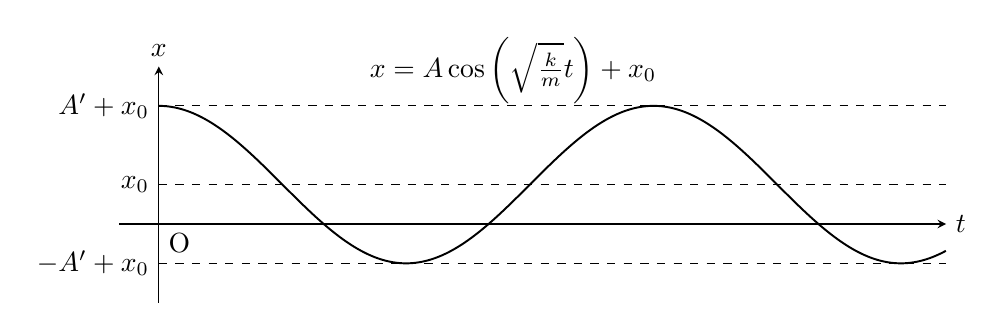
\begin{tikzpicture}[domain=-0:10,samples=300,>=stealth]
   % 座標軸
   \draw[->] (-0.5,0) -- (10,0) node[right] {$t$};
   \draw[->] (0,-1) -- (0,2) node[above] {$x$};
   \node [anchor=north west] at (0,0) {O};
 
   \draw[line width=0.7pt] plot (\x,{sin((\x+pi/2) * 180 / pi)+0.5});
   \node [anchor=north] at (4.5,2.5){$x = A\cos\left(\sqrt{\frac{k}{m}}t\right) + x_0$};
   
   % 補助線
   \draw [dashed](0,1.5) node [anchor=east]{$A'+x_0$}--(10,1.5);
   %\draw [dashed](pi/2-0.5,1.5)--(pi/2-0.5,0.8) node [below]{$\sqrt{\frac{m}{k}}\left(\frac{\pi}{2}-\theta_0\right)$};
   \draw [dashed](0,-0.5) node [anchor=east]{$-A'+x_0$}--(10,-0.5);
   \draw [dashed](0,0.5) node [anchor=east]{$x_0$}--(10,0.5);
 
\end{tikzpicture}
\caption{単振動}
\end{center}
\end{figure}





\subsection{速度の1乗に比例する抗力が働く運動型}
\label{vel_1}
次に解く運動方程式はこちらです。

\begin{equation}
    m\ddot{z} = -m'g - k\dot{z} \notag
\end{equation}

これは流体中を自然に落下する物体に関する運動方程式です。$z$を使ったのは単にこの運動が鉛直方向に起こる運動だからです。詳細は省きますが、$m'$は浮力も考慮した物体の質量で、また、誘導質量\footnote{流体の中を落下する物体は、一部の流体を加速させます。それによって本来は運動方程式が多少複雑になり、結局、見かけ上物体の慣性質量$m$が多少増加したようになります。}は無視します。

さて、これも解きやすいように変形しましょう。

\begin{equation}
    \ddot{z} = -\frac{m'}{m}g - \frac{k}{m}\dot{z} \notag
\end{equation}

これも例によって特殊解を見つけましょう。$\dot{z}$はなにかの定数で、$\ddot{z}$は$0$であると考えやすいです。そうすると$z$は$t$の1次式となって、$z=-m'gt/k + C (Cは任意定数)$はこの方程式を満たす特殊解です。そこで、$z = z' - m'gt/k + C$と置くと、

\begin{equation}
    \ddot{z'} =-\frac{k}{m}\dot{z'} \notag
\end{equation}

この方程式は睨んでも$Ae^{\gamma t}$で置いても、結局$z'$を指数関数で置換することになりそうです。仮に$z'=Ae^{\gamma t}$と置くと、

\begin{eqnarray}
    A\gamma^2 e^{\gamma t} &=& -A\gamma\frac{k}{m}e^{\gamma t} \notag \\
    \gamma &=& -\frac{k}{m} \notag
\end{eqnarray}

簡単に$\gamma$が求まります。よって、

\begin{equation}
    z = Ae^{-\frac{k}{m}t} - \frac{m'g}{k}t + C 
\end{equation}

となります。

$A<0$での$v-t$グラフ、$z-t$グラフの概形を掲載します。


\if0
\begin{figure}[!ht]
  \centering
  \includegraphics[width=12cm]{vel1_v.PNG}
  \caption{速度1乗比例の抗力が働く落下の$v-t$グラフ}
  \label{fig:vel1_v}
\end{figure}

\begin{figure}[!ht]
  \centering
  \includegraphics[width=12cm]{vel1_z.PNG}
  \caption{速度1乗比例の抗力が働く落下の$z-t$グラフ}
  \label{fig:vel1_z}
\end{figure}
\fi

\begin{figure}[htbp]
\begin{center}
\begin{tikzpicture}[domain=-0:10,samples=300,>=stealth]
   % 座標軸
   \draw[->] (-0.5,0) -- (10,0) node[right] {$t$};
   \draw[->] (0,-4) -- (0,0.5) node[above] {$v$};
   \node [anchor=north east] at (0,0) {O};
 
   \draw[line width=0.7pt] plot (\x,{3*e^(-0.4*\x)-3});
   \node [anchor=north] at (4.5,-1){$v = -A\frac{k}{m}e^{\frac{k}{m}t}-\frac{m'g}{k}$};
   
   % 補助線
   \draw [dashed](0,-3) node [anchor=east]{$-\frac{m'g}{k}$}--(10,-3);
 
\end{tikzpicture}
\caption{速度1乗比例の抵抗が働く落下 $v-t$図}
\end{center}
\end{figure}

\begin{figure}[htbp]
\begin{center}
\begin{tikzpicture}[domain=-0:10,samples=300,>=stealth]
   % 座標軸
   \draw[->] (-0.5,0) -- (10,0) node[right] {$t$};
   \draw[->] (0,-4) -- (0,2.5) node[above] {$z$};
   \node [anchor=north east] at (0,0) {O};
 
   \draw[line width=0.7pt] plot (\x,{-e^(-0.4*\x)-0.5*\x+2});
   \node [anchor=north] at (4.5,-1.3){$z = Ae^{-\frac{k}{m}t} - \frac{m'g}{k}t + C$};
   
   % 補助線
   \draw [dashed](0,1) node [anchor=east]{$-A+C$};
   \draw [dashed](0,2) node [anchor=east]{$C$}--(10,-3);
 
\end{tikzpicture}
\caption{速度1乗比例の抵抗が働く落下 $z-t$図}
\end{center}
\end{figure}



\subsection{速度の2乗に比例する抗力が働く運動型}
\label{vel_2}
今回解く運動方程式はこちらです。

\begin{equation}
    m\ddot{z} = -m'g + k\dot{z}^2 \notag
\end{equation}

速度の1乗に比例する抗力が働く運動型と酷似していますが、よく見ると$\dot{z}$の次数が2です。なんとこれは非線形の微分方程式です。しかし、これは解くことができます。

まずは$\dot{z}=v$として式を書き直しましょう。こうすることで運動方程式は1階微分方程式となり、解く方針が見えやすく鳴ります。

\begin{equation}
    m\frac{\mathrm{d}v}{\mathrm{d}t} = -m'g + kv^2 \notag
\end{equation}

$v$を左辺に、$t$を右辺に残すように変数分離し、部分分数分解し、そして積分しましょう。

\begin{eqnarray}
    -\frac{m\ \mathrm{d}v}{m'g - kv^2} &=& \mathrm{d}t \notag \\
    -\left(\frac{1}{\sqrt{m'g}-\sqrt{k}v}+\frac{1}{\sqrt{m'g}+\sqrt{k}v}\right)\frac{m\ \mathrm{d}v}{2\sqrt{m'g}} &=& \mathrm{d}t \notag \\
    -\frac{m}{2\sqrt{m'g}}\int\left(\frac{1}{\sqrt{m'g}-\sqrt{k}v}+\frac{1}{\sqrt{m'g}+\sqrt{k}v}\right)\mathrm{d}v &=& \int \mathrm{d}t \notag \\
    -\frac{m}{2\sqrt{m'g}}\log\frac{\sqrt{m'g}+\sqrt{k}v}{\sqrt{m'g}-\sqrt{k}v} &=& t + C \ (Cは任意定数) \notag \\
    \frac{\sqrt{m'g}+\sqrt{k}v}{\sqrt{m'g}-\sqrt{k}v} &=& e^{-\frac{2\sqrt{m'g}}{m}t+C'} \ (C'=-\frac{2\sqrt{m'g}}{m}C) \notag
\end{eqnarray}

ここで、物体は常に自然に落下していることから$m\ddot{z} = -m'g + k\dot{z}^2 < 0$です。これより、$\log$内は必ず正です。この式を$v$について整理すると、以下のようになります。

\begin{eqnarray}
    v &=& -\sqrt{\frac{m'g}{k}}\frac{e^{-2\frac{\sqrt{m'g}}{m}t+C'}-1}{e^{-2\frac{\sqrt{m'g}}{m}t+C'}+1} \notag \\
      &=& -\sqrt{\frac{m'g}{k}}\frac{e^{-\frac{\sqrt{m'g}}{m}t+\frac{1}{2}C'}-e^{-\frac{\sqrt{m'g}}{m}t+\frac{1}{2}C'}}{e^{-\frac{\sqrt{m'g}}{m}t+\frac{1}{2}C'}+e^{-\frac{\sqrt{m'g}}{m}t+\frac{1}{2}C'}} \notag \\
      &=& -\sqrt{\frac{m'g}{k}}\tanh\left(\frac{\sqrt{m'g}}{m}t+\theta_0\right) \ (\theta_0=\frac{1}{2}C')
\end{eqnarray}

ここで出てきた$\tanh$は双曲線関数と呼ばれ、以下に定義されます。定義を見ればお分かりの通り、指数関数をまとめて表記できるようにしただけです。

\begin{equation}
    \cosh x = \frac{e^x+e^{-x}}{2},\  \sinh x = \frac{e^x-e^{-x}}{2}, \ \tanh x = \frac{\sinh x}{\cosh x} \notag
\end{equation}

また、三角関数と似た名前というだけあって、$\cos^2 x + \sin^2 x = 1$に酷似する関係$\cosh^2 x - \sinh^2 x = 1$や、微分した際の相互関係

\begin{equation}
    \frac{\mathrm{d}}{\mathrm{d}x}\cosh x = \sinh x, \ \frac{\mathrm{d}}{\mathrm{d}x}\sinh x = \cosh x \notag
\end{equation}

があります。

それぞれの関数のグラフは以下の通りです。

\if0
\begin{figure}[!ht]
  \centering
  \includegraphics[width=15cm]{hyperbolic.PNG}
  \caption{双曲線関数のグラフ}
  \label{fig:hyperbolic}
\end{figure}
\fi
\begin{figure}[htbp]
\begin{center}
\begin{tikzpicture}[domain=-3:3,samples=300,>=stealth]
   % 座標軸
   \draw[->] (-3,0) -- (3,0) node[right] {$t$};
   \draw[->] (0,-4) -- (0,4) node[above] {$z$};
   \node [anchor=north west] at (0,0) {O};
 
   \draw[line width=1pt, domain=-2:2, dotted] plot (\x,{cosh(\x)});
   \node [anchor=north] at (-2.2,2){$y=\cosh x$};
   \draw[line width=0.7pt, domain=-2:2] plot (\x,{sinh(\x)});
   \node [anchor=north] at (-2.5,-2){$y=\sinh x$};
   \draw[line width=0.7pt, domain=-3:3, dashed] plot (\x,{tanh(\x)});
   \node [anchor=north] at (-2,-0.3){$y=\tanh x$};
   
   % 補助線
   \draw [dashed](0,1) node [anchor=south east]{$1$};
   \draw [dashed](0,-1) node [anchor=east]{$-1$};
 
\end{tikzpicture}
\caption{双曲線関数のグラフ}
\end{center}
\end{figure}

さて、本題に戻りましょう。これで$v=\dot{z}$が$t$の関数として表せました。あとはこれを$t$で積分すれば解が導けます。まずは積分の準備です。

\begin{eqnarray}
    \dot{z} &=& -\sqrt{\frac{m'g}{k}}\tanh\left(\frac{\sqrt{m'g}}{m}t+\theta_0\right) \notag \\
            &=& -\sqrt{\frac{m'g}{k}}\frac{\sinh\left(\frac{\sqrt{m'g}}{m}t+\theta_0\right)}{\cosh\left(\frac{\sqrt{m'g}}{m}t+\theta_0\right)} \notag \\
            &=& -\sqrt{\frac{m'g}{k}}\frac{\left(\cosh\left(\frac{\sqrt{m'g}}{m}t+\theta_0\right)\right)'}{\cosh\left(\frac{\sqrt{m'g}}{m}t+\theta_0\right)} \notag
\end{eqnarray}

ここで最後の式で出てきた$'$はカッコ内の関数を$t$で微分したことを示します。これで準備は整いました。$t$で積分しましょう。

\begin{eqnarray}
    \int\mathrm{d}z &=&  -\sqrt{\frac{m'g}{k}}\int\frac{\left(\cosh\left(\frac{\sqrt{m'g}}{m}t+\theta_0\right)\right)'}{\cosh\left(\frac{\sqrt{m'g}}{m}t+\theta_0\right)} \ \mathrm{d}t \notag \\
    z &=&  -\sqrt{\frac{m'g}{k}}\log\left(\cosh\left(\frac{\sqrt{m'g}}{m}t+\theta_0\right)\right) + C'' \ (C''は任意定数)
\end{eqnarray}

これでこの運動方程式が解けました。$\theta_0=0$とするときの$v-t$グラフ、$x-t$グラフは以下の通りです。

\clearpage

\begin{figure}[htbp]
\begin{center}
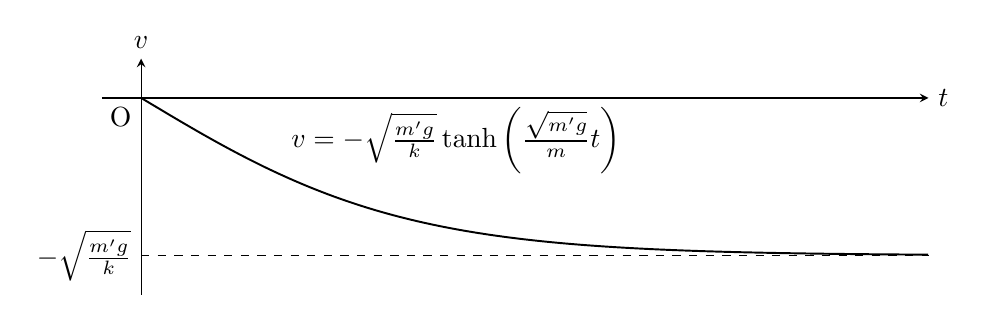
\begin{tikzpicture}[domain=0:10,samples=300,>=stealth]
   % 座標軸
   \draw[->] (-0.5,0) -- (10,0) node[right] {$t$};
   \draw[->] (0,-2.5) -- (0,0.5) node[above] {$v$};
   \node [anchor=north east] at (0,0) {O};

   \draw[line width=0.7pt, domain=0:10] plot (\x,{-2*tanh(0.3*\x)});
   \node [anchor=north] at (4,0){$v=-\sqrt{\frac{m'g}{k}}\tanh\left(\frac{\sqrt{m'g}}{m}t\right)$};

   % 補助線
   \draw [dashed](0,-2) node [anchor=east]{$-\sqrt{\frac{m'g}{k}}$}--(10,-2);
 
\end{tikzpicture}
\caption{速度2乗比例の抵抗が働く落下 $v-t$図}
\end{center}
\end{figure}

\begin{figure}[htbp]
\begin{center}
\begin{tikzpicture}[domain=0:10,samples=300,>=stealth]
   % 座標軸
   \draw[->] (-0.5,0) -- (10,0) node[right] {$t$};
   \draw[->] (0,-3) -- (0,3) node[above] {$z$};
   \node [anchor=north east] at (0,0) {O};

   \draw[line width=0.7pt, domain=0:8.5] plot (\x,{-2*ln(cosh(0.3*\x))+1});
   \node [anchor=north] at (5,2.5){$z=-\sqrt{\frac{m'g}{k}}\log\left(\cosh\left(\frac{\sqrt{m'g}}{m}t\right)\right) + C''$};

   % 補助線
   \draw [dashed](0,1) node [anchor=east]{$C''$};
   \draw [dashed](0,{2*ln(2)+1}) node [anchor=east]{$\sqrt{\frac{m'g}{k}}\log 2$}--(8.5,{-2*(0.3*8.5-ln(2))+1});
 
\end{tikzpicture}
\caption{速度2乗比例の抵抗が働く落下 $z-t$図}
\end{center}
\end{figure}




\subsection{減衰振動型}
\label{vibration+vel_1}
さて、ここからは応用です。今度解く運動方程式は以下です。

\begin{equation}
    m\ddot{x} = -k(x-x_0) - k'\dot{x} \notag
\end{equation}

これは速さの1乗に比例する抗力と復元力が働く場合の物体の運動方程式です。現実では粘性の高い流体の中でバネにおもりをつないで振動させると起こりますが、詳しくは後々お話します。ここではこの運動方程式を解くことを念頭にしましょう。$\ddot{x}$の係数を1にするように両辺$m$で割っておきましょう。

\begin{equation}
    \ddot{x} = -\frac{k}{m}(x-x_0) - \frac{k'}{m}\dot{x} \notag
\end{equation}

まずは例によって特殊解を見つけます。$x$を定数関数とすると$\dot{x},\ddot{x}$が$0$になるので都合が良いでしょう。この条件で考えると$x=x_0$は特殊解です。定石通りに$x=x'+x_0$として、

\begin{equation}
    \ddot{x'} = -\frac{k}{m}x' - \frac{k'}{m}\dot{x'} \notag
\end{equation}

と変形でき、斉次微分方程式になりました。

ここで、$\gamma \in \mathbb{C}$として$x'=Ae^{\gamma t}$と置きます。そうすると、

\begin{eqnarray}
    A\gamma^2e^{\gamma t} &=& -A\frac{k}{m}e^{\gamma t} - A\gamma\frac{k'}{m}e^{\gamma t} \notag \\
    \gamma^2 &=& -\frac{k}{m} - \frac{k'}{m}\gamma \notag 
\end{eqnarray}

これは$\gamma$についての2次方程式です。この解は以下です。

\begin{eqnarray}
    \gamma &=& \frac{1}{2}\left(-\frac{k'}{m} \pm \sqrt{\frac{k'^2}{m^2}-4\frac{k}{m}}\right) \notag \\
           &=& \frac{1}{2}\left(-\frac{k'}{m} \pm \sqrt{\mu-\kappa}\right) \notag
\end{eqnarray}

後の都合のため、判別式を簡単に置換しました。このまま解としても良いですが、これは判別式$D$の$0$との比較によって場合分けをしてもう少し変形したほうがわかりやすそうです。

\begin{enumerate}
    \item $D\geq 0 \Leftrightarrow \mu \geq \kappa$\\
             $\gamma\in\mathbb{R}$で、$\frac{1}{2}\sqrt{D}$を$\gamma'$として、2つの解$x'$を定数倍して足し合わせると、
            
            \begin{eqnarray}
                x' &=& c_1 e^{\left(-\frac{k'}{2m}+\gamma'\right)t} + c_2 e^{\left(-\frac{k'}{2m}-\gamma'\right)t} \notag \\
                   &=& e^{-\frac{k'}{2m}t}\left(c_1e^{\gamma't}+c_2e^{-\gamma't}\right) \notag
                   %&=& A'e^{-\frac{k'}{2m}t}\cosh(\gamma't) \ (A' = 2A) \notag
            \end{eqnarray}
            
             よって、
            
            \begin{equation}
                x=e^{-\frac{k'}{2m}t}\left(c_1e^{\gamma't}+c_2e^{-\gamma't}\right)+x_0
                %x = A'e^{-\frac{k'}{2m}t}\cosh(\gamma't) + x_0 \notag
            \end{equation}
            
             少し考察してみましょう。$D\geq 0 \Leftrightarrow \mu \geq \kappa$は簡単に考えると、速度の1乗に比例する抗力と物体にかかる復元力をある指標で比べた時に、抗力が特に大きいことを示しています。実際、直感の通り、$D\geq 0$の条件の下では、詳細は省きますが、$x$は一定値$x_0$に収束します。また、$D>0$の状態は過減衰、$D=0$の状態は臨界減衰と言います。グラフを見ればお分かりの通り、臨界減衰が一番早く$x$が収束し、$D$が大きくなるにつれて収束までの時間が長くなっていきます。これは単に、減衰(抵抗)が大きすぎると、物体が$x=x_0$に戻るにも抵抗が邪魔をして戻りにくくなっている状態を表します。いくつか$D$の値を調整した$x-t$グラフを載せましょう。グラフは上から$D=0.8,0.6,0$です。
            
            
            
            \begin{figure}[htbp]
            \begin{center}
            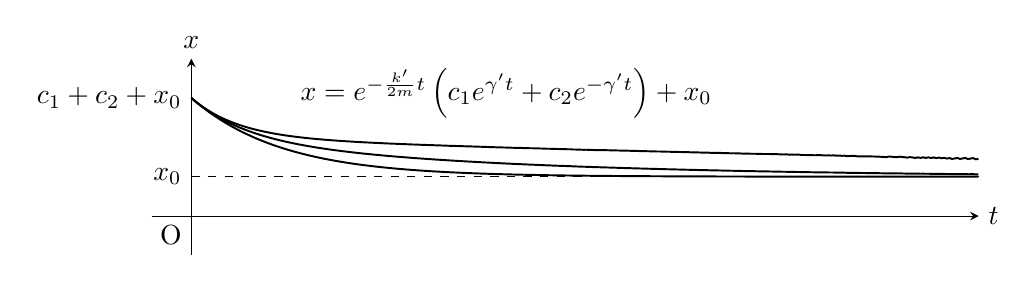
\begin{tikzpicture}[domain=0:10,samples=300,>=stealth]
               % 座標軸
               \draw[->] (-0.5,0) -- (10,0) node[right] {$t$};
               \draw[->] (0,-0.5) -- (0,2) node[above] {$x$};
               \node [anchor=north east] at (0,0) {O};
               
               \draw[line width=0.7pt, domain=0:10] plot (\x,{e^(-0.7/0.8*\x)*cosh(0.8*\x)+0.5});
               \draw[line width=0.7pt, domain=0:10] plot (\x,{e^(-0.7/0.8*\x)*cosh(0.6*\x)+0.5});
               \draw[line width=0.7pt, domain=0:10] plot (\x,{e^(-0.7/0.8*\x)*cosh(0*\x)+0.5});
               \node [anchor=north] at (4,2){$x=e^{-\frac{k'}{2m}t}\left(c_1e^{\gamma't}+c_2e^{-\gamma't}\right)+x_0$};
            
               % 補助線
               \draw [dashed](0,0.5) node [anchor=east]{$x_0$}--(10,0.5);
               \draw [dashed](0,1.5) node [anchor=east]{$c_1+c_2+x_0$};
             
            \end{tikzpicture}
            \caption{減衰振動(過減衰)}
            \end{center}
            \end{figure}
            
            
            
    \item $D < 0\Leftrightarrow \mu < \kappa$ \\
             $\gamma\in\mathbb{C}\cap\overline{\mathbb{R}}$ですから、オイラーの公式を使うことになりそうです。$\frac{1}{2}\sqrt{D}$を$\gamma'\mathrm{i}$として、2つの解を定数倍して足すと、
            
            \begin{eqnarray}
                x' &=& c_1e^{\left(-\frac{k'}{2m}+\gamma'\mathrm{i}\right)t} + c_2e^{\left(-\frac{k'}{2m}-\gamma'\mathrm{i}\right)t} \notag \\
                   &=& e^{-\frac{k'}{2m}t}\left(c_1 e^{\gamma'\mathrm{i}t}+c_2 e^{-\gamma'\mathrm{i}t}\right) \notag \\
                   &=& e^{-\frac{k'}{2m}t}\left((c_1+c_2)\cos(\gamma't)+(c_1-c_2)\mathrm{i}\sin(\gamma't)\right) \notag 
            \end{eqnarray}
            
             初期条件$t=0$で$x=A+x_0$かつ$\dot{x}=v(\in\mathbb{R})$として、代入するために$x$を$t$で微分して、
             
            \begin{eqnarray}
                \dot{x} = e^{-\frac{k'}{2m}t}\left(\left(\gamma'(c_1-c_2)\mathrm{i}-\frac{k'}{2m}(c_1+c_2)\right)\cos(\gamma't)-\left(\frac{k'}{2m}(c_1-c_2)\mathrm{i}+\gamma'(c_1+c_2)\right)\sin(\gamma't)\right) \notag
            \end{eqnarray}
            
             ですから、
             
            \begin{eqnarray}
                x(t=0) &=& c_1+c_2+x_0 \ (=A+x_0) \notag \\
                \dot{x}(t=0) &=& \gamma'(c_1-c_2)\mathrm{i}-\frac{k'}{2m}(c_1+c_2) \ (=v) \notag
            \end{eqnarray}
            
             よって、$c_1+c_2=A$かつ$c_1-c_2=0$がわかります。なお、$k'A/(2m)=v$という関係もわかりました。
            
             これより、結局$x$は、
            
            \begin{equation}
                x = Ae^{-\frac{k'}{2m}t}\cos(\gamma't)+ x_0
                \label{eq:decayvibration}
            \end{equation}
            
             と表せます。
            
             また少し考察をしましょう。$D < 0\Leftrightarrow \mu < \kappa$は簡単に考えると、速度の1乗に比例する抗力と物体にかかる復元力をある指標で比べた時に復元力が特に大きいことを示しています。実際、グラフは振動しながら$x=x_0$に収束していきます。
            
             $x-t$グラフを載せましょう。
            \if0
            \begin{figure}[!ht]
              \centering
              \includegraphics[width=12cm]{vib_vel1_2.PNG}
              \caption{復元力と速度1乗比例の抗力が働く運動の$x-t$グラフ(減衰振動)}
              \label{fig:vib_vel1_2}
            \end{figure}
            \fi
            
            \begin{figure}[htbp]
            \begin{center}
            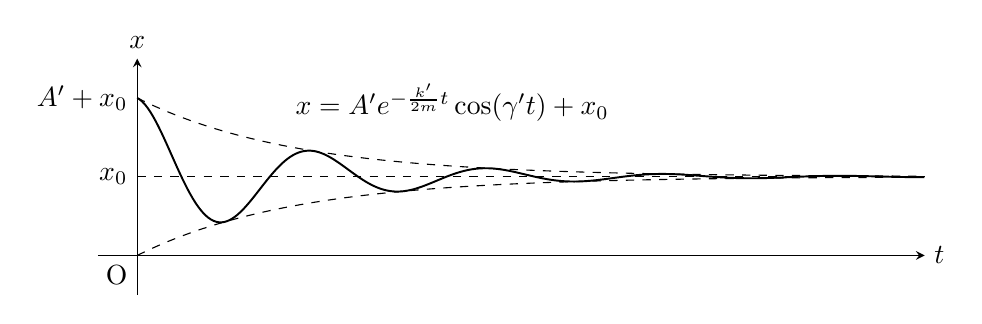
\begin{tikzpicture}[domain=0:10,samples=300,>=stealth]
               % 座標軸
               \draw[->] (-0.5,0) -- (10,0) node[right] {$t$};
               \draw[->] (0,-0.5) -- (0,2.5) node[above] {$x$};
               \node [anchor=north east] at (0,0) {O};
            
               \draw[line width=0.7pt, domain=0:10] plot (\x,{e^(-0.4/0.8*\x)*cos(2.8*180/pi*\x)+1});
               \node [anchor=north] at (4,2.3){$x = A'e^{-\frac{k'}{2m}t}\cos(\gamma't)+ x_0$};
               \draw[dashed, domain=0:10] plot (\x,{1+e^(-0.4/0.8*\x)});
               \draw[dashed, domain=0:10] plot (\x,{1-e^(-0.4/0.8*\x)});
               %\node [anchor=north] at (4,0.9){$x = -A'e^{-\frac{k'}{2m}t}+x_0$};
               % 補助線
               \draw [dashed](0,1) node [anchor=east]{$x_0$}--(10,1);
               \draw [dashed](0,2) node [anchor=east]{$A'+x_0$};
             
            \end{tikzpicture}
            \caption{減衰振動(振動)}
            \end{center}
            \end{figure}
\end{enumerate}



\subsection{減衰系の強制振動型}
\label{forcedvibration}
最後に解く運動方程式は以下です。これは減衰振動する物体に外力を加えて強制振動させることを表す式です。

\begin{eqnarray}
    m\ddot{x}=-kx-k'\dot{x}+F \notag
\end{eqnarray}

ここで、$F$は$t$の関数とします。

これを整理すると、

\begin{eqnarray}
    \ddot{x}+\frac{k}{m}x+\frac{k'}{m}\dot{x}=\frac{1}{m}F \notag
\end{eqnarray}

まずは$F$を具体的な何かの関数で置きましょう。物理でなにか関数で置くと言ったら指数関数か三角関数ですね\footnote{そうでない場合はなかなか解けません}。今回は物体を強制的に振動させることを考えるので、$F=f\cos(\omega t)$とします。

すると、運動方程式は

\begin{eqnarray}
    \ddot{x}+\frac{k}{m}x+\frac{k'}{m}\dot{x}=\frac{1}{m}f\cos(\omega t) \notag
\end{eqnarray}

となります。

次に定石通り特殊解を探しましょう。今回は右辺が$t$の関数となっているので、$x$を定数関数や1次関数としてもうまくいきそうにありません。そこで、$x=A\cos(\omega t + \theta_0)$と置いてみましょう。加法定理で分解して、$A$について整理してみましょう。

\begin{eqnarray}
    -A\omega^2\cos(\omega+\theta_0)+\frac{k}{m}A\cos(\omega t+\theta_0)-\frac{k'}{m}A\omega\sin(\omega t+\theta_0)&=&\frac{f}{m}\cos(\omega t) \notag \\
    -A\omega^2(\cos(\omega t)\cos\theta_0-\sin(\omega t)\sin\theta_0) \notag\\
    +\frac{k}{m}A(\cos(\omega t)\cos\theta_0-\sin(\omega t)\sin\theta_0) \notag\\
    -\frac{k'}{m}A\omega(\sin(\omega t)\cos\theta_0+\cos(\omega t)\sin\theta_0) &=& \frac{f}{m}\cos(\omega t) \notag \\
    \cos(\omega t)\left(-A\omega^2\cos\theta_0+\frac{k}{m}A\cos\theta_0-\frac{k'}{m}A\omega\sin\theta_0\right)\notag\\
    +\sin(\omega t)\left(A\omega^2\sin\theta_0-\frac{k}{m}A\sin\theta_0-\frac{k'}{m}A\omega\cos\theta_0\right)&=&\frac{f}{m}\cos(\omega t) \notag
\end{eqnarray}

このとき、右辺と左辺が一致するには、左辺で$(\sin(\omega t)の係数)=0$かつ$(\cos(\omega t)の係数)=f/m$です(そうでないと両辺の位相が一致しません)。

前者の条件から、両辺を$A\cos\theta_0$で割って$\tan\theta_0$について整理して、

\begin{eqnarray}
    A\omega^2\sin\theta_0-\frac{k}{m}A\sin\theta_0-\frac{k'}{m}A\omega\cos\theta_0&=&0 \notag \\
    \omega^2\tan\theta_0-\frac{k}{m}\tan\theta_0-\frac{k'}{m}\omega&=&0 \notag \\
    \tan\theta_0&=&\frac{k'\omega}{m\omega^2-k} \notag
\end{eqnarray}

$1+\tan^2\theta=1/\cos^2\theta$と$\sin^2\theta+\cos^2\theta=1$を使って$\cos\theta,\sin\theta$を求めると、

\begin{eqnarray}
    \cos\theta_0 &=& \sqrt{\frac{1}{1+\tan^2\theta_0}} \notag \\
    &=&\sqrt{\frac{(m\omega^2-k)^2}{(m\omega^2-k)^2+(k'\omega)^2}} \notag \\
    &=&\frac{m\omega^2-k}{\sqrt{(m\omega^2-k)^2+(k'\omega)^2}} \notag
\end{eqnarray}

\begin{eqnarray}
    \sin\theta_0 &=& \sqrt{1-\cos^2\theta} \notag \\
    &=&\sqrt{\frac{(k'\omega)^2}{(m\omega^2-k)^2+(k'\omega)^2}} \notag \\
    &=&\frac{k'\omega}{\sqrt{(m\omega^2-k)^2+(k'\omega)^2}} \notag
\end{eqnarray}

また、後者の条件と$\sin\theta_0,\cos\theta_0$から、

\begin{eqnarray}
    -A\omega^2\cos\theta_0+\frac{k}{m}A\cos\theta_0-\frac{k'}{m}A\omega\sin\theta_0&=&\frac{f}{m} \notag \\
    A\left(\left(-\omega^2+\frac{k}{m}\right)\cos\theta_0-\frac{k'}{m}\omega\sin\theta_0\right)&=&\frac{f}{m} \notag \\
    A\left(\left(-\omega^2+\frac{k}{m}\right)\frac{m\omega^2-k}{\sqrt{(m\omega^2-k)^2+(k'\omega)^2}}-\frac{k'}{m}\omega\frac{k'\omega}{\sqrt{(m\omega^2-k)^2+(k'\omega)^2}}\right)&=&\frac{f}{m} \notag
\end{eqnarray}

\begin{eqnarray}
    A\left(\left(-\omega^2+\frac{k}{m}\right)(m\omega^2-k)-\frac{k'}{m}\omega k'\omega\right)&=&\frac{f}{m}\sqrt{(m\omega^2-k)^2+(k'\omega)^2} \notag \\
    A\left(-(m\omega^2-k)^2-(k'\omega)^2\right)&=&f\sqrt{(m\omega^2-k)^2+(k'\omega)^2} \notag \\
    A&=&-\frac{f}{\sqrt{(m\omega^2-k)^2+(k'\omega)^2}} \notag
\end{eqnarray}

さて、これで特殊解が求まりました。これと減衰振動の一般解(式(\ref{eq:decayvibration}))から、この運動方程式の一般解は

\begin{eqnarray}
    x=A'e^{-\frac{k'}{2m}t}\cos(\gamma't)-\frac{f}{\sqrt{(m\omega^2-k)^2+(k'\omega)^2}}\cos(\omega t+\theta_0)
    \label{eq:forcedvibration}
\end{eqnarray}

と表せます。このグラフは以下の通りです。

\clearpage

\begin{figure}[htbp]
\begin{center}
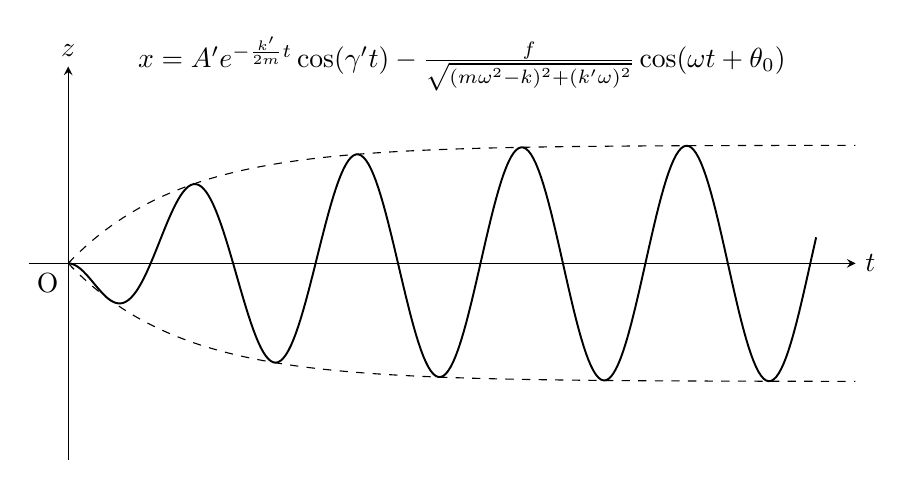
\begin{tikzpicture}[domain=0:10,samples=300,>=stealth]
   % 座標軸
   \draw[->] (-0.5,0) -- (10,0) node[right] {$t$};
   \draw[->] (0,-2.5) -- (0,2.5) node[above] {$z$};
   \node [anchor=north east] at (0,0) {O};

   \draw[line width=0.7pt, domain=0:9.5] plot (\x,{e^(-0.7*\x)*1.5*sin(3*\x*180/pi)-1.5*sin(3*\x*180/pi)});
   \node [anchor=north] at (5,3){$x=A'e^{-\frac{k'}{2m}t}\cos(\gamma't)-\frac{f}{\sqrt{(m\omega^2-k)^2+(k'\omega)^2}}\cos(\omega t+\theta_0)$};
   \draw[dashed, domain=0:10] plot (\x,{1.5*(1-e^(-0.7*\x))});
   \draw[dashed, domain=0:10] plot (\x,{-1.5*(1-e^(-0.7*\x))});
   
 
\end{tikzpicture}
\caption{減衰系の強制振動}
\end{center}
\end{figure}

さて、ここで少し考察してみましょう。$t\rightarrow\infty$のとき、式(\ref{eq:forcedvibration})での右辺第一項は$0$となります。よって、周期的な外力を加えて物体を振動させる場合、最終的に物体は右辺第二項(つまり特殊解)の動きをします。このとき、$\omega$を動かして$|A|$、つまり十分時間が経ったときの振幅を見てみましょう。

\begin{figure}[htbp]
\begin{center}
\begin{tikzpicture}[domain=0:10,samples=300,>=stealth]
   % 座標軸
   \draw[->] (-0.5,0) -- (10,0) node[right] {$\omega$};
   \draw[->] (0,-0.5) -- (0,3) node[above] {$A$};
   \node [anchor=north east] at (0,0) {O};

   \draw[line width=0.7pt, domain=0:9.5] plot (\x,{6/sqrt((\x^2-6)^2+(\x)^2)});
   \draw [dashed]({sqrt(6)},0) node [anchor=north] {$\sqrt{\frac{k}{m}}$} -- ({sqrt(6)},2.5);
\end{tikzpicture}
\caption{$\omega$と$A$の関係}
\end{center}
\end{figure}

図を見ると、$\omega=\sqrt{k/m}$周辺で$A$が最大値を取っていることがわかります。この$\omega_0=\sqrt{k/m}$を物体の固有振動数と言います。

余談ですが、固有振動数に関しては怖い事故も起きています。とある橋では風によってうまく固有振動数に近い力が与えられて大きく揺れ、最後には崩れてしまいました。またある橋では、通行人が橋を渡るときにかかる力の周期が固有振動数に近くて、大きく揺れてしまいました。またある建物では、ダンスをしていたらたまたま固有振動数に近い周期の力を与えてしまったがために床が落ちてしまいました。